%! TEX root = ./main.tex

\lecture{4}{Week: 2}{Continue Integers}

\subsubsection{Sign extension}
Given a $w$ bit signed integer $x$, convert it to a $w + k$ bit signed integer with the same value.

We do that by copying the most significant bit of $x$ and copy it to all $k$ new bits.

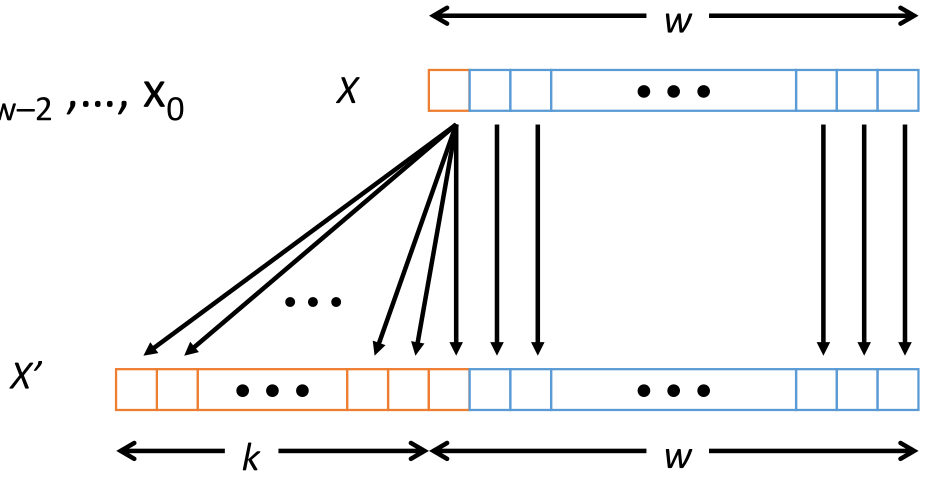
\includegraphics[width=0.8\textwidth]{04_signExtend.png}

For unsigned numbers, the number is padded with zeros at the beginning.

C does this sign extend automatically for us.

\subsubsection{Truncation}
Throws away the left bits. For unsigned numbers it represents the modulo operator. For signed integers it is also like modulo, but it does it in a special way (negative number may get positive and vice versa).

Also, only small numbers remain unchanged.

\subsubsection{Addition and Subtraction in C}
\paragraph{Negation}
Number $x$ can be negated using $\tilde x + 1 == -x$.

It follows that $\tilde x + x == 111 \dots 111 == -1$

\paragraph{Unsigned addition}
When adding two unsigned numbers $u$ and $v$ of length $w$, we get a number of length $w + 1$.

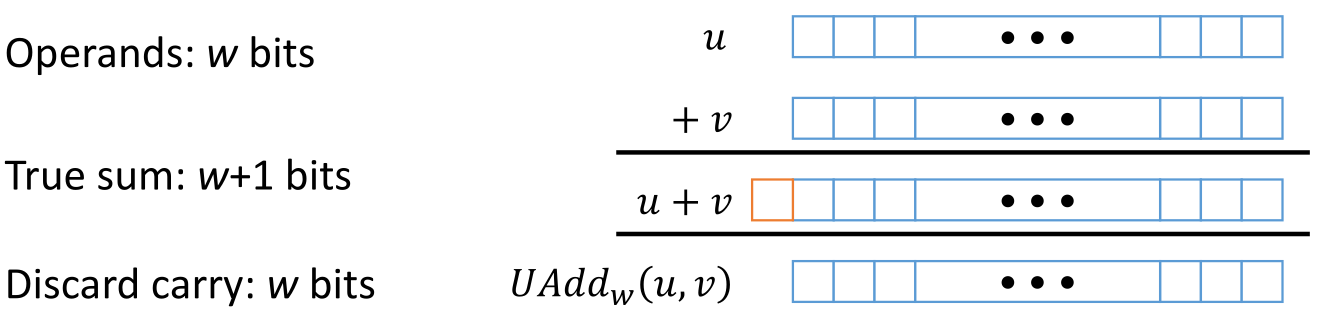
\includegraphics[width=0.8\textwidth]{04_unsignedAdditionEquation.png}

The function $UAdd_w(u,v)$ ignores the extra bit which would be required if the sum overflows the $w$ bits. This function can also be seen as:

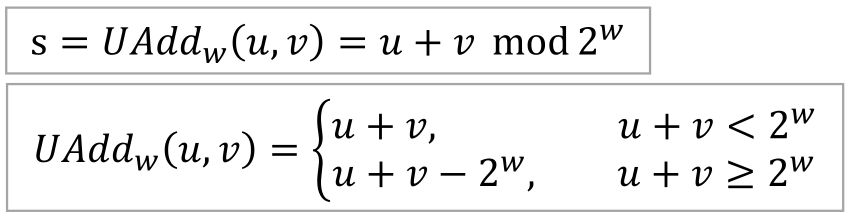
\includegraphics[width=0.8\textwidth]{04_unsignedAdditionFormula.png}

Then the sum overflows, it wraps around.

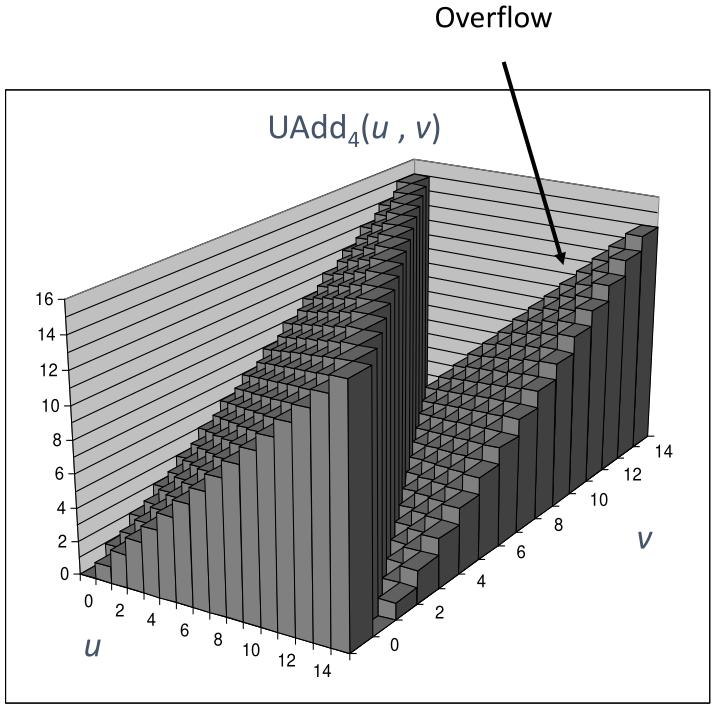
\includegraphics[width=0.8\textwidth]{04_01_unsignedAddition.png}

The $Uadd_w$ function is the classical unsigned addition operator in C. There are certain compilers which provide some possibility to retrieve a possible overflow.

$UAdd_w(u,v)$ is an Abelian group (Closed, Commutative, Associative, Identity, Inverse)

\paragraph{Two's complement addition}
When adding two signed numbers $u$ and $v$ of length $w$, we get a number of length $w + 1$.

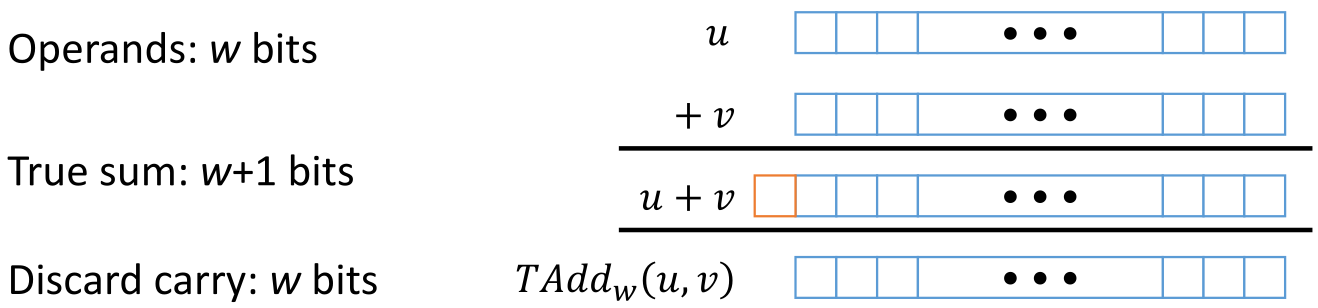
\includegraphics[width=0.8\textwidth]{04_signedAdditionEquation.png}

The function $TAdd_w(u,v)$ ignores the extra bit which would be required if the sum overflows the $w$ bits.

$TAdd_w(u,v)$ behaves identical to $UAdd$ in the bit level interpretation. But the overflow behaves differently (are interpreted differently). Positive overflow gives a negative number, a negative overflow gives a positive number.

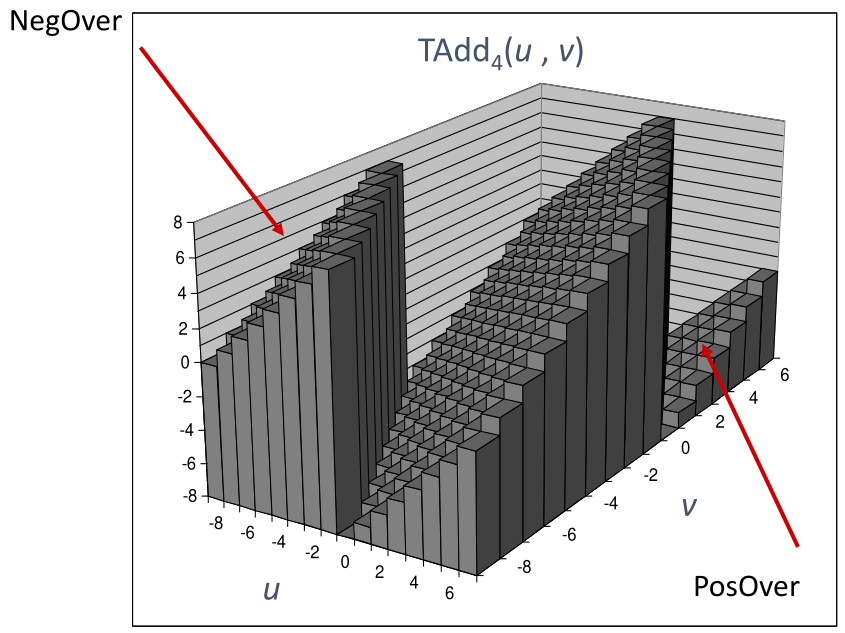
\includegraphics[width=0.8\textwidth]{04_02_signedAddition.png}

The function can be seen as:

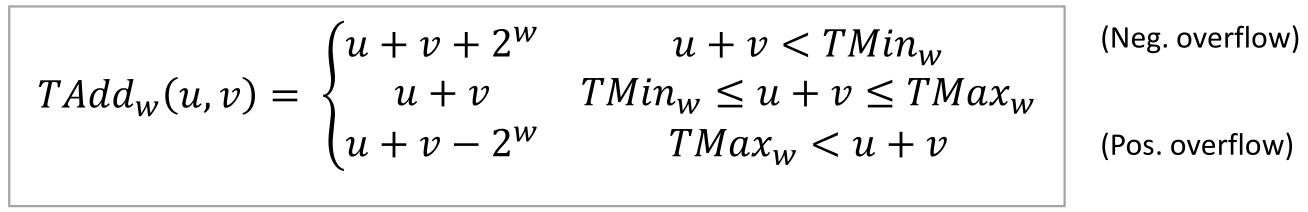
\includegraphics[width=0.8\textwidth]{04_signedAdditionFormula.png}

$TAdd$ is isomorphic to $UAdd$ and $TAdd$ forms a group (closed, commutative, associative, identity, inverse).

\subsubsection{Integer multiplication in C}

\paragraph{Unsigned Multiplication}
When multiplying two unsigned numbers $u$ and $v$ of length $w$, we get a number of length $2w$.

So, we can get all number $0 \le x \cdot y \le (2^w -1)^2$.

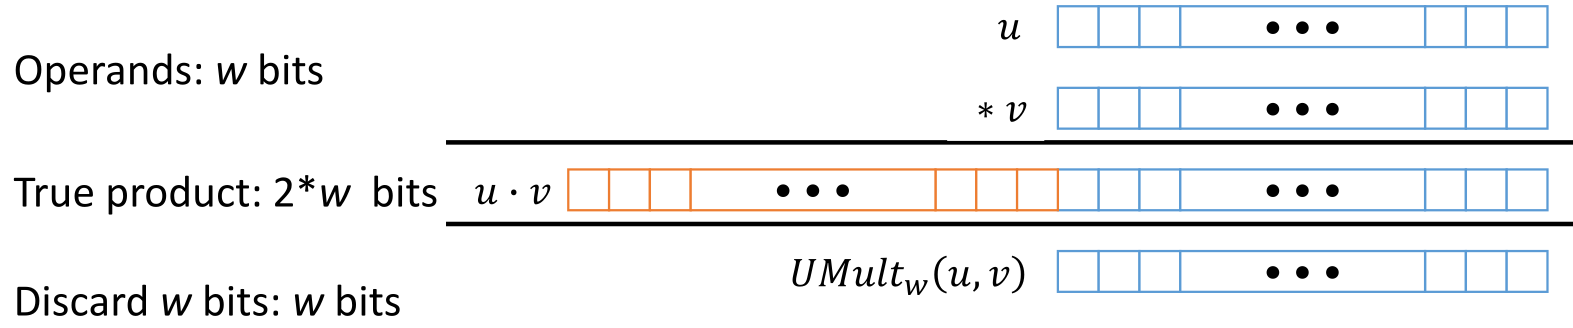
\includegraphics[width=0.8\textwidth]{04_unsignedMultiplyEquation.png}

The operator $UMult_w(u,v)$ truncates the overflowing bits. The formula can be seen as:

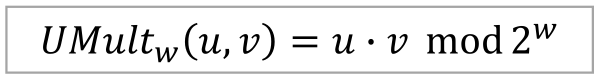
\includegraphics[width=0.8\textwidth]{04_unsignedMultiplyFormula.png}

$UMult_w$ forms a commutative ring with $UAdd$.

\paragraph{Signed Multiplication}
When multiplying two signed numbers $u$ and $v$ of length $w$, we get a number of length $2w$.

We can represent the range $(-2^{w - 1}) \cdot (2^{w - 1} - 1) \le x \cdot y \le (-2^{w -1})^2$.

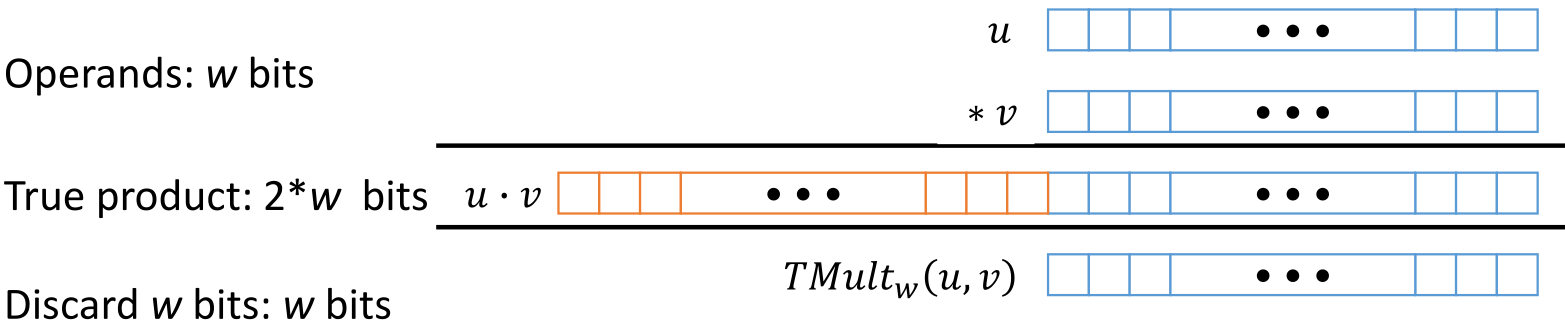
\includegraphics[width=0.8\textwidth]{04_signedMultiplicationEquation.png}

The operator $TMult_w(u,v)$ ignores the overflowing bits. Some hardware puts overflowing bits into a special register, but they are normally not accessibly in C.

\subsubsection{Multiplication and Division Using Shifts}
\paragraph{Multiplication}
As we have seen, the shift operator shifts the binary representation of a number. Regarding the interpreted number, $u << k$ results in $u \cdot 2^k$. This is valid for signed and unsigned numbers.

When shifting a signed/unsigned number of length $w$ by $k$, the $k$ overflowing bits are truncated.

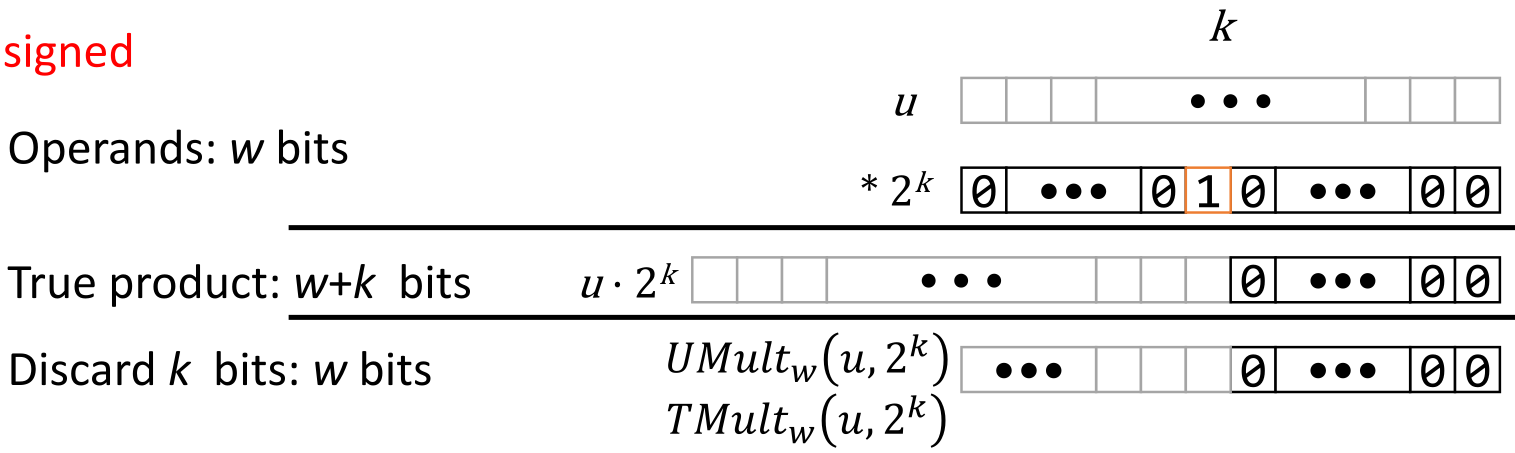
\includegraphics[width=0.8\textwidth]{04_powerOfTwo.png}

Multiplication is much more complex than simple shifts. Therefore, to calculate $u \cdot 24$ we may write $(u << 5) - (u << 3)$. But modern compiler do such things (and even better optimisations) for us, therefore we should not do it.

\paragraph{Division}
Equally as with multiplication, shifts can be used for division of power of twos. $u >> k$ gives $\lfloor \frac{u}{2^k} \rfloor$. The underflowing $k$ bits get truncated.

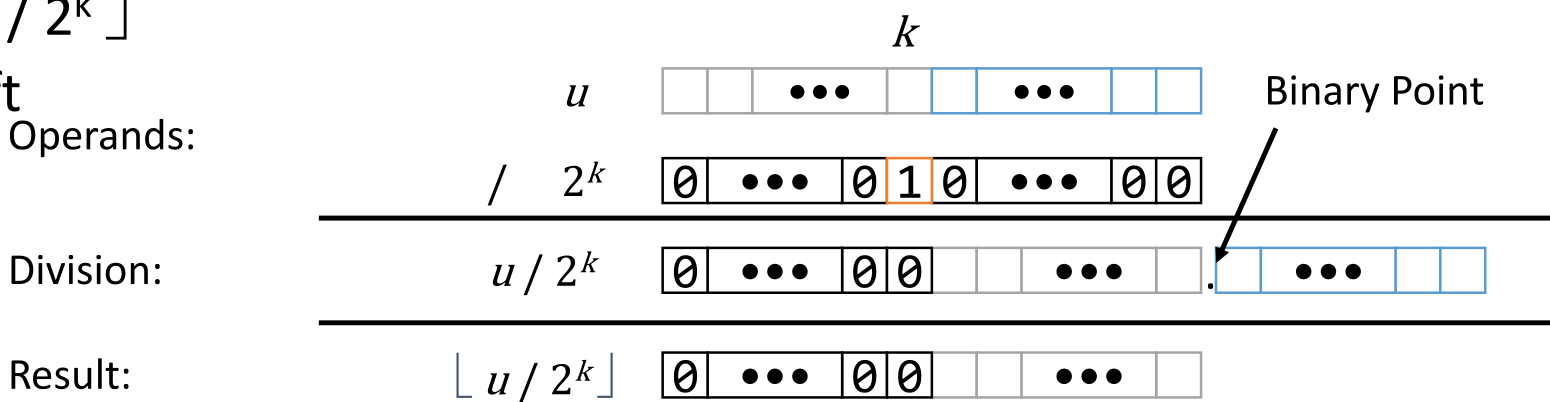
\includegraphics[width=0.8\textwidth]{04_powerOfTwoDivide.png}

Even though this works for unsigned and signed numbers, for signed numbers the results may be wrong for negative numbers.
This is because we round down, but actually we would like to round towards $0$. We can fix that by computing $\lfloor \frac{(u + 2^k - 1)}{2^k} \rfloor$. In C this is equivalent to $(u + (1 << k) -1) >> k$. This formula works for positive and negative numbers.

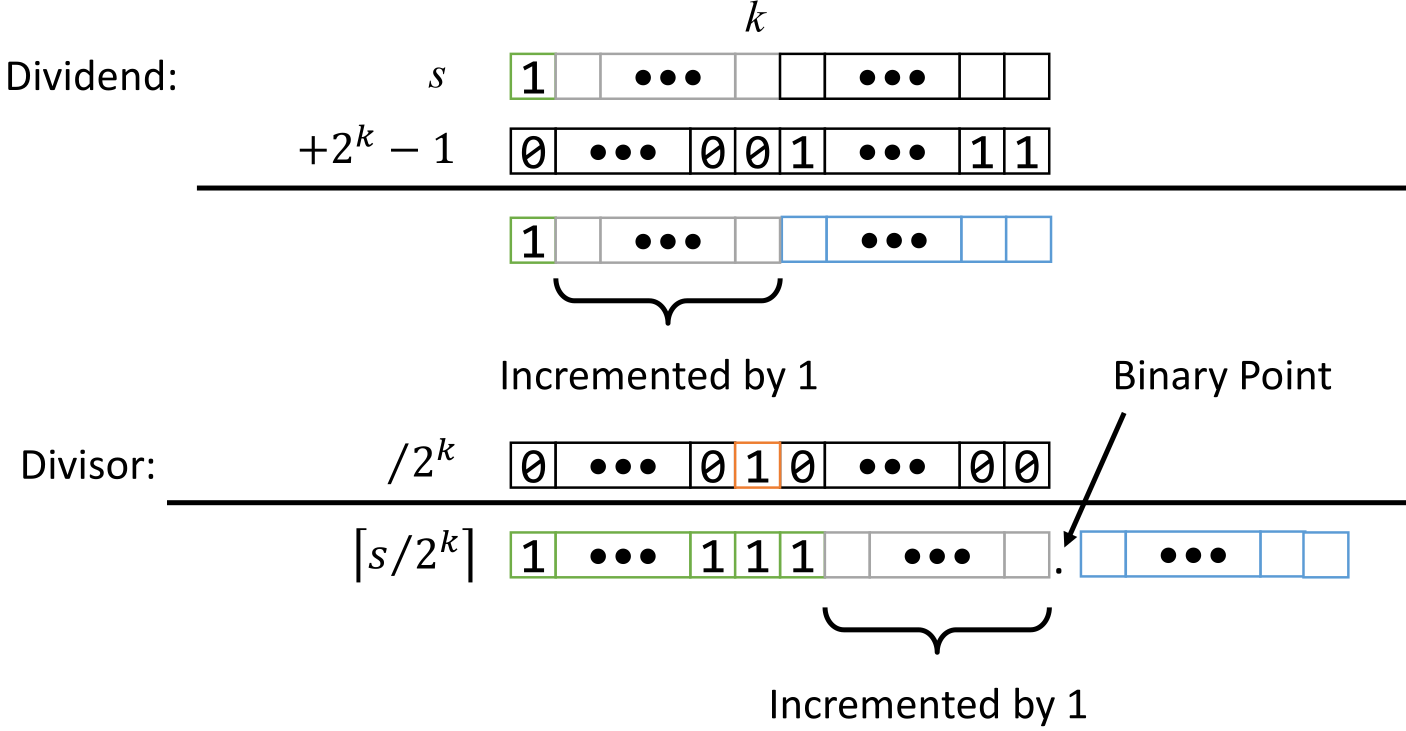
\includegraphics[width=0.8\textwidth]{04_powerOfTwoDivideCorrect.png}


Again, the compiler can translate divisions into shifts. For unsigned numbers, it applies the first formula, for signed numbers the second one.

\subsubsection{C Integer puzzles}
In the following are some integer related puzzles to solve.

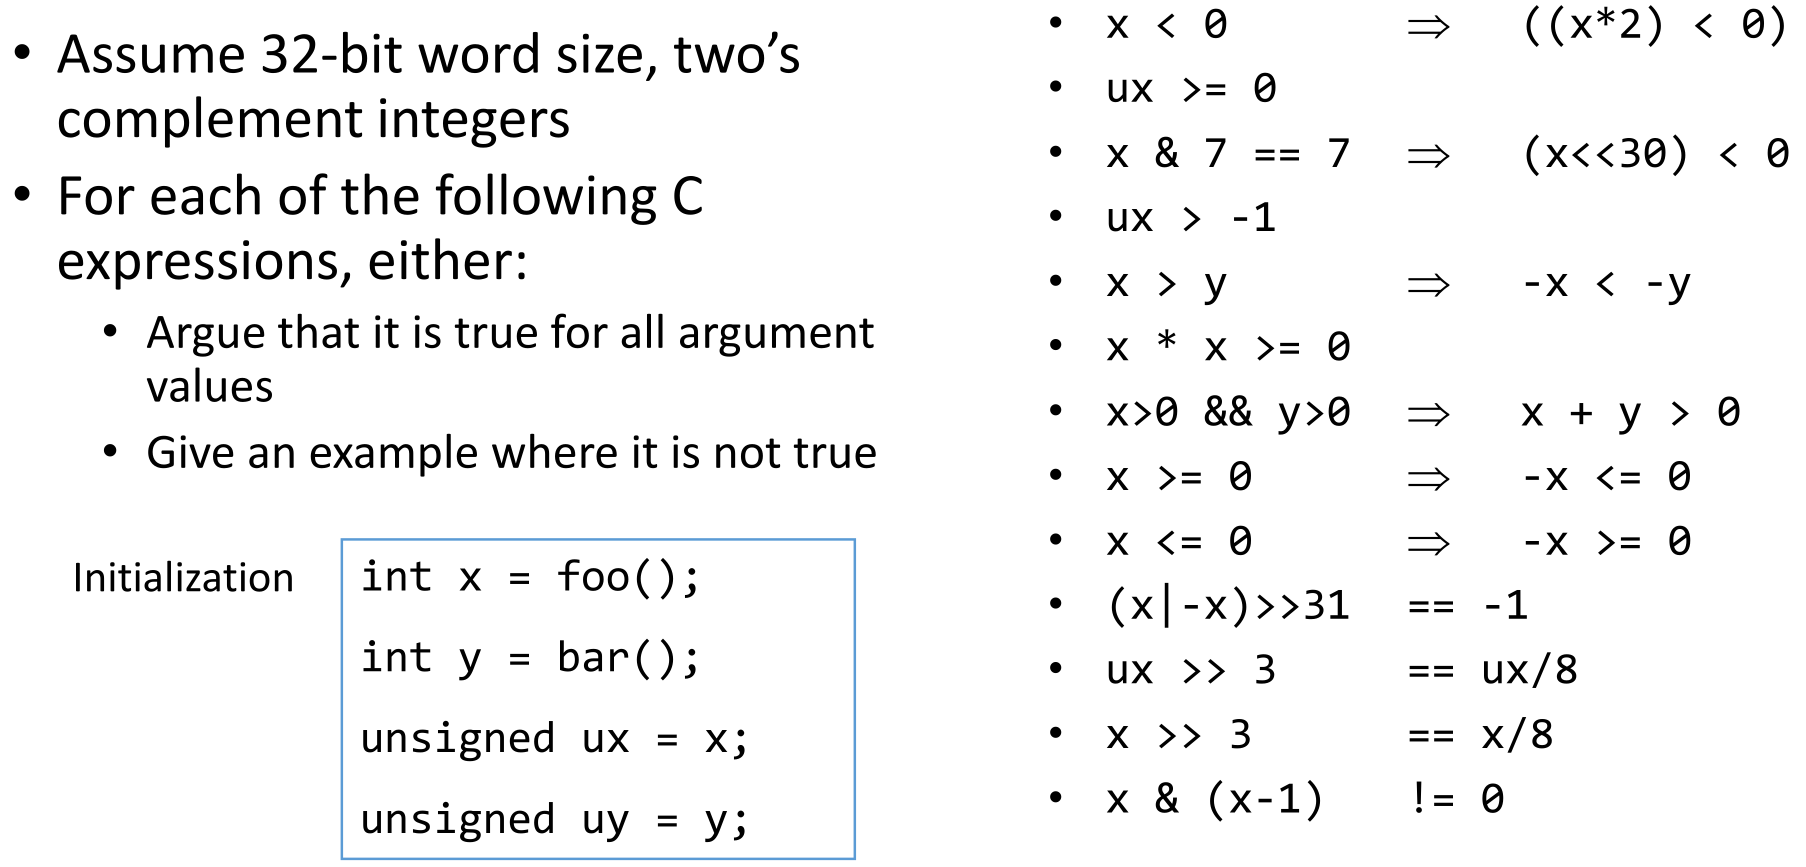
\includegraphics[width=0.8\textwidth]{04_integerPuzzle.png}
